\documentclass[12pt,fleqn,handout]{beamer}


\xdefinecolor{lavendar}{rgb}{0.8,0.6,1}
\xdefinecolor{olive}{cmyk}{0.64,0,0.95,0.4}
%\xdefinecolor{olive}{cmyk}{1,0,0,0}
\xdefinecolor{mag}{cmyk}{0.1,1,0,0.2}
\xdefinecolor{lblue}{rgb}{0,0,1.5}
\xdefinecolor{lred}{rgb}{1,0,0}
\xdefinecolor{mine}{cmyk}{1,0,0.2,0}
\xdefinecolor{bluel}{cmyk}{0.1,0,0.9,0.4}

\usepackage{amsmath,amssymb,dsfont,mathrsfs}
\usepackage{tikz,pgflibraryplotmarks}
\usepackage{multimedia}
\usepackage{wasysym}
\usepackage{rotating}
\usepackage{algorithm,algorithmic}
\usepackage{graphicx} % more modern
\usepackage{subfigure}
\usepackage{booktabs}

\usepackage{pgfplots}
\usepackage{verbatim}

\usepackage{setspace}
\newlength\iwidth
\newlength\iheight

\newcommand\makebeamertitle{\frame{\maketitle}}%
\graphicspath{{./images/}}
\setbeamertemplate{navigation symbols}{}
\addtobeamertemplate{navigation symbols}{}{%
    \usebeamerfont{footline}%
    \usebeamercolor[fg]{footline}%
	\insertshorttitle
    \;--
    \insertframenumber
}

\newcommand{\sectionstart}{
	\only<beamer>{
 	\begin{frame}% (fold)
 		\begin{centering}\Huge \insertsection \par\end{centering}
 	\end{frame}% frame the_application (end)
	}
 }


% make bibliography entries smaller
\usepackage{natbib}
\setbeamertemplate{bibliography item}{[\theenumiv]}
\renewcommand\bibfont{\scriptsize}
\setbeamertemplate{frametitle continuation}[from second]
\newcommand{\tcr}{\textcolor{red}}
\newcommand{\tcrd}{\textcolor{red}}
\newcommand{\tcb}{\textcolor{bluel}}
\newcommand{\tcm}{\textcolor{mag}}
\newcommand{\tcg}{\textcolor{olive}}

\newcommand{\R}{\mathbb{R}}
\newcommand{\C}{\mathbb{C}}

% bold lower-case for vectors
\newcommand{\bfa}{{\bf a}}
\newcommand{\bfb}{{\bf b}}
\newcommand{\bfc}{{\bf c}}
\newcommand{\bfs}{{\bf s}}
\newcommand{\bfm}{{\bf m}}
\newcommand{\bfd}{{\bf d}}
\newcommand{\bfe}{{\bf e}}
\newcommand{\bfu}{{\bf u}}
\newcommand{\bfy}{{\bf y}}
\newcommand{\bfx}{{\bf x}}
\newcommand{\bfh}{{\bf h}}
\newcommand{\bfw}{{\bf w}}
\newcommand{\bfv}{{\bf v}}
\newcommand{\bfr}{{\bf r}}
\newcommand{\bfz}{{\bf z}}
\newcommand{\bfp}{{\bf p}}


% bold upper-case for linear operators
\newcommand{\bfA}{{\bf A}}
\newcommand{\bfB}{{\bf B}}
\newcommand{\bfZ}{{\bf Z}}
\newcommand{\bfM}{{\bf M}}
\newcommand{\bfC}{{\bf C}}
\newcommand{\bfD}{{\bf D}}
\newcommand{\bfQ}{{\bf Q}}
\newcommand{\bfJ}{{\bf J}}
\newcommand{\bfG}{{\bf G}}
\newcommand{\bfI}{{\bf I}}
\newcommand{\bfP}{{\bf P}}
\newcommand{\bfK}{{\bf K}}
\newcommand{\bfY}{{\bf Y}}
\newcommand{\bfW}{{\bf W}}
\newcommand{\bfR}{{\bf R}}
\newcommand{\bfL}{{\bf L}}
\newcommand{\bfF}{{\bf F}}
\newcommand{\bfT}{{\bf T}}
\newcommand{\bfS}{{\bf S}}
\newcommand{\bfX}{{\bf X}}
\newcommand{\bfU}{{\bf U}}
\newcommand{\bfV}{{\bf V}}
\newcommand{\bfH}{{\bf H}}


\newcommand{\calF}{\mathcal{F}}



\newcommand{\hf}{{\frac 12}}
\newcommand{\bftheta}{{\boldsymbol \theta}}
\newcommand{\bfxi}{{\boldsymbol \xi}}

\newcommand{\bfLambda}{{\boldsymbol \Lambda}}
\newcommand{\bfSigma}{{\boldsymbol \Sigma}}
\newcommand{\bfepsilon}{{\boldsymbol \epsilon}}

\newcommand{\E}{\vec E}
\newcommand{\B}{\vec B}

\newcommand{\vu}{  {\vec {\bf u}}}

\newcommand{\grad}{  {\vec {\bf \nabla}}}

\newcommand{\lfrownie}{\textcolor{red}{\large{\frownie}}}
\newcommand{\lsmiley}{\textcolor{green}{\large{\smiley}}}

\newcommand{\curl}{\ensuremath{\nabla\times\,}}
\renewcommand{\div}{\nabla\cdot\,}
\newcommand{\divh}{\nabla_h\cdot\,}
\renewcommand{\grad}{\ensuremath{\nabla}}

\DeclareMathOperator*{\argmin}{arg\,min}


\title{Classification}
\subtitle{Numerical Methods for Deep Learning}
\date{}
\begin{document}

\makebeamertitle

\section{Logistic Regression and Softmax} % (fold)
\label{sec:logistic_regression_and_softmax}

\begin{frame}
	\frametitle{Logistic Regression}
	
	
	Assume our data falls into two classes. Denote by $\bfc_{\rm obs}(\bfy)$ the probability that example $\bfy\in\R^{n_f}$ belongs to first category.
	
	\bigskip
	
	Since output of our classifier $f(\bfy,\theta)$ is supposed to be probability, use logistic sigmoid
	$$
		\bfc(\bfy,\theta) = \frac{1}{1 + \exp\left(-f(\bfy,\theta)\right)}.
	$$
	
	\bigskip
	
	Example (Linear Classification): If $f(\bfy,\theta)$ is a linear function (adding bias is easy), $\theta = \bfw \in \R^{n_f}$ and
	$$
		\bfc(\bfy,\bfw) = \frac{1}{1 + \exp(-\bfw^\top\bfy)}.
	$$
	
	\begin{center}
		from now on consider linear models for simplicity
	\end{center}
	
\end{frame}

\begin{frame}
	\frametitle{Multinomial Logistic Regression}
	
	Suppose data falls into $n_c\geq 2$ categories and the components of $\bfc_{\rm obs}(\bfy) \in[0,1]^{n_c}$ contain probabilities for each class. 
	
	\bigskip
	 
	Applying the logistic sigmoid to each component of $f(\bfy,\bfW)$ not enough (probabilities must sum to one). Use
	$$
		\bfc(\bfy,\bfW) = \left( \frac{1}{\bfe_{n_c}^\top\exp(\bfW\bfy)} \right) \; \exp(\bfW\bfy).
	$$
	
	\bigskip
	
	Note: Division and $\exp$ are applied element-wise!
	
\end{frame}
\begin{frame}
	\frametitle{Logistic Regression - Loss Function}
	
	How similar are $\bfc(\cdot,\bfW)$ and $\bfc_{\rm obs}(\cdot)$?
	
\bigskip

	Naive idea: Let $\bfY \in \R^{n_f\times n}$ be examples with class probabilities $\bfC_{\rm obs} \in [0,1]^{n_c\times n}$, use 
	$$
	\phi(\bfW)= \frac{1}{2n} \sum_{j=1}^n\|\bfc(\bfy_j,\bfW) - \bfc_{j,{\rm obs}} \|_F^2
	$$

Problems
\begin{itemize}
	\item ignores that $\bfc(\cdot,\bfW)$ and $\bfc_{\rm obs}(\cdot)$ are distributions.
	\item leads to non-convex objective function
\end{itemize} 

\bigskip

Need to be careful to treat $\bfc$ appropriately. 	
	
\end{frame}


\begin{frame}
	\frametitle{Example: Designing a Code}
	
	Goal: Communicate using minimal number of bits.
	
	\bigskip
	\pause
	
	\invisible<beamer|1>{
	Example: Bob talks $\bfc = [1/2,1/4,1/8,1/8]$ of the time about dogs, cats, fish, and birds, respectively.
	
	How many bits need to be transferred on average?}

	\bigskip
	
	\invisible<beamer|-2>{
	\begin{center}
		\begin{tabular}{l|cc}
			word & naive code & \invisible<beamer|-3>{better code} \\ \hline
			dog  & 00         & \invisible<beamer|-3>{ 0 }         \\ 
			cat  & 01         & \invisible<beamer|-3>{ 10   }      \\
			fish & 10         & \invisible<beamer|-3>{ 110  }      \\ 
			bird & 11         & \invisible<beamer|-3>{ 111   }     \\
		\end{tabular}		
	\end{center}
	}
	
	\invisible<beamer|-4>{
	\begin{center}
		Idea: Quantify information content in probability distribution using average length.		
	\end{center}
	}
	
	
	\only<beamer|5>{}
	

\end{frame}

\begin{frame}
	\frametitle{Entropy}

	Note: Length of word depends on its probability being used. How long should a word be?
	
	\bigskip
	\pause
	
	Optimal choice for information for any category
$$ I = \log_2(\bfc_j^{-1}) = -\log_2(\bfc_j) $$


\bigskip

The larger $\bfc_j$, the more common we use it, the shorter the word should be. 

\bigskip
\pause

The entropy is the average (expectation) of information over all classes.

$$ E(\bfc) = -\sum \bfc_j \log_2(\bfc_j) = -\bfc^{\top} \log_2(\bfc) $$

\end{frame}

\begin{frame}
	\frametitle{Example: Designing a Code - 2}

	Entropy for Bob's code is
	$$
		\frac{1}{2} \log\left(2\right) + \frac{1}{4} \log\left(4\right) + 2 \frac{1}{8} \log\left(8\right) = 1.75
	$$
	average length of word is 1.75 bits $<$ 2 bits for naive code!
	
\bigskip


\bigskip
\pause

For the complete tutorial on entropy, read
{\small
\tt{http://colah.github.io/posts/2015-09-Visual-Information/}
}

\end{frame}

\begin{frame}
	\frametitle{Properties of Entropy}

\begin{itemize}
\item recall $\lim_{x\rightarrow 0} x \log x = 0$
\item prefer sparse distributions (why?)
\item has been used in compressed sensing type methods
\end{itemize}

\begin{center}
\begin{figure}
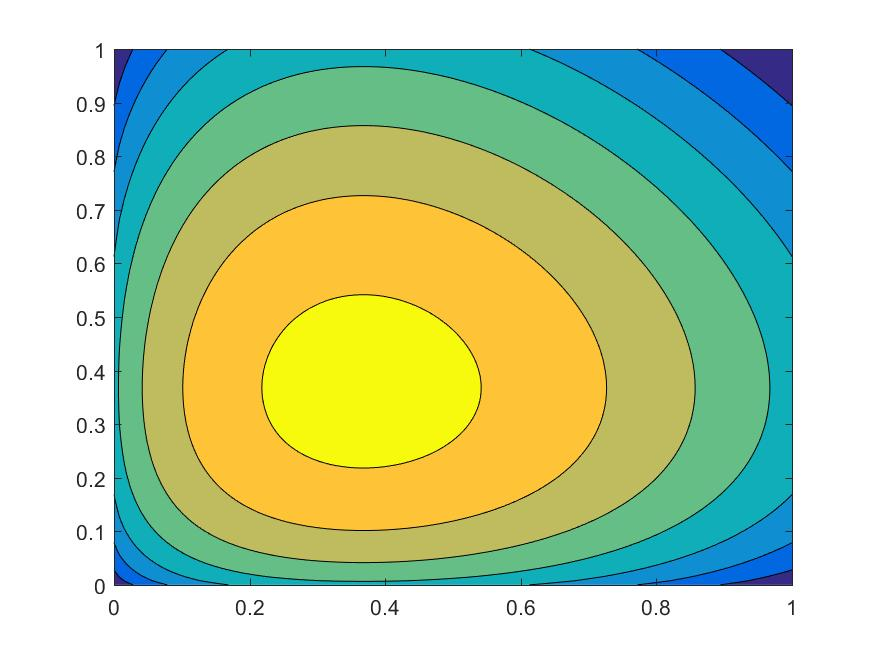
\includegraphics[width=5cm]{entropy.jpg}
\caption{The entropy of a vector $\bfc = (c_1, c_2)^\top$}
\end{figure}
\end{center}


\end{frame}

\begin{frame}
	\frametitle{Cross Entropy}


Measure the average word length when using code designed for $\bfc$ for sending information with probability $\widehat \bfc$
$$ E(\widehat\bfc, \bfc) = - {\widehat \bfc}^{\top} \log(\bfc). $$

\bigskip

Clearly
$$ E(\widehat\bfc,  \bfc) \ge E(\bfc, \bfc) $$

\bigskip
\pause

Example: Alice talks $\bfc = [1/8,1/2,1/4,1/8]$ of the time about dogs, cats, fish, and birds, respectively.
If she used Bob's code, the average word length would be 
$$
	\frac{1}{8} \log\left(2\right) + \frac{1}{2} \log\left(4\right) + \frac{1}{4} \log\left(8\right) + \frac{1}{8} \log\left(8\right) = 2.25 > 1.75
$$

\bigskip
\pause

$E$ measures how similar the distributions $\bfc$ and $\widehat \bfc$ are.


\bigskip
\pause

One flaw: $ E(\bfc, \widehat \bfc) \not= E(\widehat \bfc, \bfc)$ (verify for our example!)


\end{frame}

\begin{frame}
	\frametitle{Cross Entropy for Logistic Regression - 1}

Recall: For a single example and two classes we have
 $$
  \bfc(\bfy,\bfw)  = \begin{pmatrix}
  	{\frac 1 {1+\exp(-\bfw^{\top} \bfy)}} \\
	1-{\frac 1 {1+\exp(-\bfw^{\top} \bfy)}}
  \end{pmatrix} 
  \stackrel{\rm def}{=} 
  \begin{pmatrix}
  	h(\bfw^{\top}\bfy) \\1-h(\bfw^{\top}\bfy)
  \end{pmatrix}
 $$

Assume we have the observation $\bfc_{\rm obs} = \begin{pmatrix}
	\bfc_{\rm obs} \\ 1-\bfc_{\rm obs}
\end{pmatrix}$ then
\begin{align*}
 E(\bfc_{\rm obs}, \bfc) & = -\bfc_{\rm obs}^\top\log(\bfc(\bfy,\bfw)) \\
 & = -\bfc_{\rm obs} \log(h(\bfw^{\top}\bfy)) - (1-\bfc_{\rm obs})
\log(1-h(\bfw^{\top}\bfy)). 
\end{align*}
where
$$
 h(z) = \frac{1}{1+\exp(-z)}
$$
\end{frame}

\begin{frame}
	\frametitle{Cross Entropy for Logistic Regression - 2}


In the case we have many examples need to sum over the data
\begin{align*}
	\bfC(\bfY,\bfw) & = \begin{pmatrix}
		{\frac 1 {1+\exp(-\bfw^\top \bfY)}} \\
		1-{\frac 1 {1+\exp(\bfw^\top\bfY)}}
	\end{pmatrix}  \stackrel{def}{=} \begin{pmatrix}
		h(\bfw^\top \bfY)\\ 1-h(\bfw^\top\bfY)
	\end{pmatrix}
	\in \R^{2\times n}
\end{align*}
Assume we have the observation $\bfc_{\rm obs}\in\R^n$. Define
$$
\bfC_{\rm obs} = \begin{pmatrix}
	\bfc_{\rm obs}^\top \\ 1-\bfc_{\rm obs}^\top
\end{pmatrix} \in \R^{2 \times n}.
$$

Then the cross entropy is
\begin{align*}
	E(\bfC_{\rm obs}, \bfC)  =& - \frac{1}{n} {\rm tr}(\bfC_{\rm obs}^\top \bfC) \\
	 						 = & -\frac{1}{n} \bfc_{\rm obs}^{\top} \log(h(\bfw^\top\bfY) \\
							   & - \frac{1}{n}(1-\bfc_{\rm obs})^{\top}\log(1-h(\bfw^\top\bfY)))
\end{align*}

\end{frame}

\begin{frame}
	\frametitle{Cross Entropy for Multinomial Logistic Regression}
	
	Similarly, for general case ($n_c\geq2$ classes, $n$ examples). 
	
	Recall: 
	$$\bfC(\bfY,\bfW)  =   \exp(\bfW \bfY) {\rm diag} \left({\frac 1 {\bfe_{n_c}^\top\exp(\bfW \bfY)}}  \right)  $$

\bigskip

Get cross entropy by summing over all examples

$$ E(\bfC_{\rm obs},\bfC(\bfY,\bfW)) = -\frac{1}{n}{\rm tr}( \bfC_{\rm obs}^\top\log(\bfC(\bfY,\bfW)) ). $$

We will also call this the \emph{softmax} (cross-entropy) function.


\end{frame}


\begin{frame}\frametitle{Simplifying the Softmax Function}

Let $\bfS = \bfW \bfY$, then 
$$ 
E(\bfC_{\rm obs},\bfS) = -\frac{1}{n}{\rm tr}\left(\bfC_{\rm obs}^{\top} \log\left({\exp(\bfS)}{\rm diag}\left(\frac{1}{\bfe_{n_c}^\top \exp(\bfS) }\right) \right)\right). 
$$

Verify that this is equal to
\begin{align*}
	 E(\bfC_{\rm obs},\bfS) = & -\frac{1}{n}\bfe_{n_c}^{\top} \left( \bfC_{\rm obs} \odot \bfS\right) \bfe_{n} \\
	 & + \frac{1}{n} \bfe_{n_c}^\top \bfC_{\rm obs}\log\left(\bfe_{n_c}^\top\exp(\bfS)\right)^\top
\end{align*}
($\odot$ is Hadamard product, $\exp$ and $\log$ component-wise)
\bigskip
\pause


If $\bfC_{\rm obs}$ has a unit row sum (why?) then $ \bfe_{n_c}^\top \bfC_{\rm obs}^\top = \bfe_n^\top$
and 
$$ E(\bfC_{\rm obs},\bfS) = -\frac{1}{n}\bfe_{n_c}^{\top} \left( \bfC_{\rm obs} \odot \bfS\right) \bfe_{n} 
+ \frac{1}{n}\log(\bfe_{n_c}^\top\exp(\bfS))\bfe_{n} $$


\end{frame}



\begin{frame}\frametitle{Numerical Considerations}

Scale to prevent overflow. Note that for an arbitrary $s\in\R$ we have
$$ E(\bfC_{\rm obs},\bfW\bfY-s) = E(\bfC_{\rm obs},\bfW\bfY) $$

This prevents overflow, but may lead to underflow (and divisions by zero).

\bigskip
\pause

Note that $s$ does not need to be the same in each row (example). Hence, 
we can choose $\bfs = \max(\bfW\bfY,[],1 ) \in \R^{1\times n}$ to avoid underflow and overflow.

\bigskip
\begin{center}
For stability use $E(\bfC_{\rm obs},\bfS)$ where $ \bfS = \bfW \bfY - \bfe_{n_c} \bfs$.
\end{center}
\end{frame}

\begin{frame}[fragile]\frametitle{Test Problem: Linear Classification}

Generate data that is linearly separable:

\begin{center}
	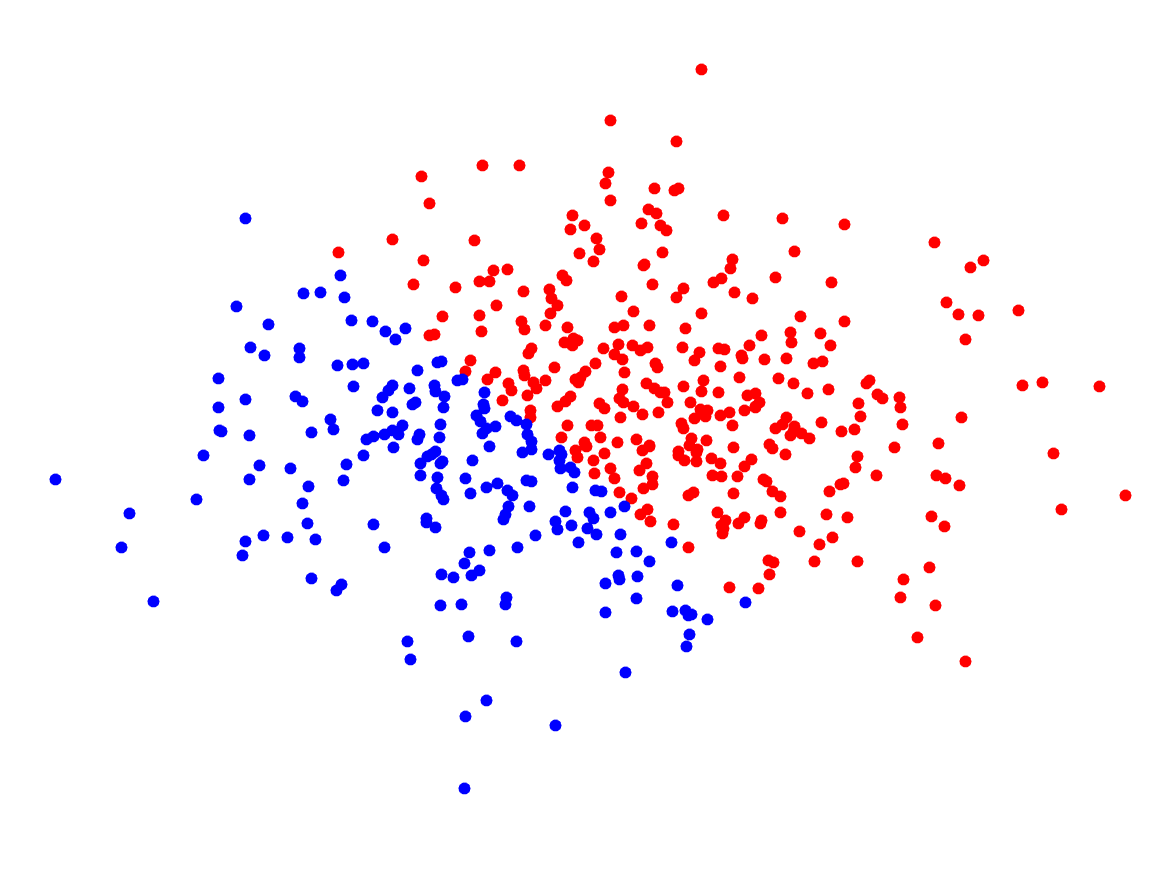
\includegraphics[height=40mm]{linearClass}
\end{center}
\vspace*{-5mm}
\begin{verbatim}

a = 3; b = 2;

Y = randn(2,500);
C = a*Y(1,:) + b*Y(2,:) + 1;
C(C>0) = 1; C(C<0) = 0;
C = [C; 1-C]

\end{verbatim}


\end{frame}


\begin{frame}[fragile]\frametitle{Coding: Softmax Regression Objective Function}


Write a function that computes the softmax function given a data matrix $\bfY$,
its class $\bfC$, and a matrix $\bfW$.

\bigskip

\begin{verbatim}
function[E] = softmaxFun(W,Y,C)

% Your code here


end
\end{verbatim}
\begin{center}
	Test your code using \texttt{testSoftmax.m}
\end{center}
\end{frame}


\begin{frame}\frametitle{Linear Classification}

If $\bfW$ can separate the classes then the goal is to minimize the cross entropy (with some potential regularization)

\begin{align*}
 \bfW^* = & \argmin_{\bfW} \quad - \frac{1}{n}\bfe_{n_c}^{\top} \left( \bfC_{\rm obs} \odot \bfS\right) \bfe_{n} 
+ \frac{1}{n} \log(\bfe_{n_c}^\top \exp(\bfS))\bfe_n \\
          & \text{subject to} \;\bfS = \bfW \bfY - \bfe_{n_c} \bfs
\end{align*}
\pause

This is a smooth convex optimization problem \\ $\Rightarrow$ many existing optimization techniques will work

\bigskip

For large-scale problems, use derivative-based optimization algorithm. (Examples: Steepest Descent, Newton-like methods,  Stochastic Gradient Descent, \ldots)

\bigskip

Excellent references: \cite{NocedalWright2006,BoydVandenberghe2004,Beck2014}
\end{frame}


\begin{frame}\frametitle{Differentiating the Softmax Regression Function}

We need to compute the derivative of the cross entropy function with respect to $\bfW$.
Three hints:
\begin{itemize}
\item $\sum \bfw \odot \bfy = \bfw^{\top} \bfy $
\item $\grad_{\bfw} (\bfw^{\top} \bfy) = \bfy$
\item ${\rm vec} (\bfW \bfY) = (\bfY^\top \otimes \bfI) {\rm vec} (\bfW) = (\bfI \otimes \bfW) {\rm vec}(\bfY)$
\end{itemize}
where $\otimes$ is the Kronecker product.

\bigskip



We use the common notation:
\begin{itemize}
	\item ${\rm vec}(\bfA)$ reshapes matrix $\bfA$ (column-wise) into vector
	\item ${\rm mat}(\bfa)$ reshapes vector $\bfa$ into matrix, ${\rm mat}({\rm vec}(\bfA)) = \bfA$.
	\item ${\rm diag}(\bfA) = {\rm diag}({\rm vec}( \bfA))$ builds diagonal matrix with entries given by $\bfA$. 
\end{itemize}


\end{frame}

\begin{frame}[fragile]\frametitle{Differentiating the Softmax Function}

Do it in three steps:
\begin{enumerate}
	\item $\nabla_{\bfS} E(\bfS)$ with $\bfS = \bfY \bfW$ (assume w.l.o.g. no shift)
	\item $\nabla_{\bfW} \bfS = \nabla_{\bfW} (\bfW \bfY)$
	\item use chain rule to get $\nabla_{\bfW} E(\bfW\bfY)$.
\end{enumerate}

\bigskip
\pause

Break the first step down into two terms
$$ E(\bfS) = \frac{1}{n} \overbrace{-{\rm tr}(\bfC_{\rm obs}^{\top} \bfS)}^{E1} + \frac{1}{n} \overbrace{\log(\bfe_{n_c}\exp(\bfS))\bfe_n}^{E2}, $$


\bigskip
\pause

First term is linear

$$\grad_{\bfS}E_1 =  \grad_{\bfS} {\rm tr}(\bfC_{\rm obs}^{\top} \bfS) = \bfC_{\rm obs}. $$

\end{frame}

\begin{frame}[fragile]\frametitle{Differentiating the Softmax Function}


$$ E(\bfS) = \frac{1}{n}\overbrace{-{\rm tr}(\bfC_{\rm obs}^{\top} \bfS)}^{E1} + \frac{1}{n} \overbrace{\log(\bfe_{n_c}^\top\exp(\bfS))\bfe_n}^{E2}  $$


\bigskip

Second  term requires a bit more care

$$ \bfJ_{\bfS}E_2 = \bfJ_{\bfS} \bfe_n^{\top}\log(\bfe_{n_c}^\top \exp(\bfS)) = 
 \bfe_n^{\top}\bfJ_{\bfS}  \log(\bfe_{n_c}^\top\exp(\bfS))  $$

\pause 
 and
 
$$ \bfJ_{\bfS}  \log(\bfe_{n_c}^\top\exp(\bfS)) = {\rm diag}
\left( {\frac {1}{\bfe_{n_c}^\top\exp(\bfS)}}\right)
\bfJ_{\bfS}\left(\bfe_{n_c}^\top\exp(\bfS) \right) $$
 

\end{frame}


\begin{frame}[fragile]\frametitle{Differentiating the Softmax Function}
	Recall:
$$ \bfJ_{\bfS}  E_2 = \bfe_n^\top  {\rm diag}
\left( {\frac {1}{\bfe_{n_c}^\top\exp(\bfS)}}\right)
\bfJ_{\bfS}\left(\bfe_{n_c}^\top\exp(\bfS) \right) $$

Focus on last term:
\begin{align*}
   \bfJ_{\bfS} (\bfe_{n_c}^\top \exp(\bfS)) & = \bfJ_{\bfS} \left(\left(\bfI \otimes \bfe_{n_c}^{\top} \right)  {\rm vec}(\exp(\bfS))\right)\\
   &  = (\bfI \otimes \bfe_{n_c}^{\top})  {\rm diag}( {\rm vec}(\exp(\bfS)))
\end{align*}
 
 \pause
 Putting it together
 
 
 $$ \bfJ_{\bfS}E_2 =  \bfe_n^{\top}\ {\rm diag}
\left( {\frac {1}{\bfe_{n_c}^\top \exp(\bfS)}}\right) \  ( \bfI \otimes \bfe_{n_c}^{\top})  {\rm diag}( {\rm vec}(\exp(\bfS))) $$


\pause

\begin{center}
	Left to do: Take transpose
\end{center}


\end{frame}

\begin{frame}[fragile]\frametitle{Differentiating the Softmax Function}

 
 $$ \grad_{\bfS}E_2 =     {\rm diag}( {\rm vec}(\exp(\bfS))) (\bfI \otimes \bfe_{n_c})
  {\rm diag}
\left( {\frac {1}{\bfe_{n_c}^\top\exp(\bfS)}}\right) \bfe_n
     $$
\pause
simplifying

 $$ \grad_{\bfS}E_2 =     {\rm diag}( {\rm vec}(\exp(\bfS))) (\bfI \otimes \bfe_{n_c})
\left( {\frac {1}{\bfe_{n_c}^\top\exp(\bfS)}}\right)
     $$
 
\pause    
     Avoid ${\rm diag}$ and simplify using  matrix representation
     
 $$ \grad_{\bfS}E_2 =     \exp(\bfS) \odot 
\left( \bfe_{n_c} \left({\frac {1}{\bfe_{n_c}^\top \exp(\bfS)}}\right)\right) 
     $$
     
     \bigskip
     \pause
     Finally combine gradients of $E_1$ and $E_2$
     
$$     \grad_{\bfS}E =  -\frac{1}{n}\bfC_{\rm obs} + \frac{1}{n}\exp(\bfS) \odot 
\left( \bfe_{n_c} \left({\frac {1}{\bfe_{n_c}^\top \exp(\bfS)}}\right)\right) . $$
     
    

\end{frame}

\begin{frame}[fragile]\frametitle{Differentiating the Softmax Function}

$$ E(\bfW) = -\frac{1}{n}\overbrace{{\rm tr}(\bfC_{\rm obs}^{\top} (\bfW\bfY))}^{E1} + \frac{1}{n} \overbrace{\bfe_n^{\top}\log(\bfe_{n_c}^\top \exp(\bfW\bfY))}^{E2}  $$

\bigskip
Note that
$$
	\nabla_{\bfW} \bfS = \nabla_{\bfW} (\bfW \bfY) = \nabla_{\bfW} \left( (\bfY^\top \otimes \bfI) {\rm vec}(\bfW) \right) = \bfY \otimes \bfI. 
$$


\bigskip

Hence, applying the chain rule gives
     
$$     \grad_{\bfW}E = \frac{1}{n} \left( -\bfC_{\rm obs} + \exp(\bfS) \odot 
\left( \bfe_{n_c} \left({\frac {1}{\bfe_{n_c}^\top \exp(\bfS)}}\right)\right) \right)\bfY^\top. $$
     

\end{frame}


\begin{frame}[fragile]\frametitle{Coding: Differentiating the Softmax Function}

Extend your softmax function, so that it returns the gradient if needed.

\begin{verbatim}
function[E,dE] = softmaxFun(W,Y,C)

% Your code from before

if nargout > 1

% Your code for gradient here
end

end
\end{verbatim}

\end{frame}



\begin{frame}[fragile]\frametitle{Testing your Derivatives}

Your derivatives are assumed to be wrong unless you prove otherwise.

Test based on Taylor theorem. Let $\bfW$ be fixed and $\bfD$ be a random direction (same size as $\bfW$):

{\begin{small}
\begin{center}
\begin{tabular}{c|c|c}
 $h$  & $E(\bfW + h\bfD) -    E(\bfW)$ &  $E(\bfW + h\bfD) -    E(\bfW) - h {\rm tr}(\bfD^{\top} \nabla E(\bfW))$ \\
 \hline
 1   &   &   \\
 $2^{-1}$   &   &   \\
 $2^{-2}$   &   &   \\
 $2^{-3}$   &   &   \\
 $2^{-4}$   &   &   \\
 $2^{-5}$   &   &
 \end{tabular}
 \end{center}
 \end{small}}


\pause

First column should decay as ${\cal O}(h)$ \\
Second column should decay as ${\cal O}(h^2)$ \\


\end{frame}



\begin{frame}\frametitle{Derivative-Based Optimization: Steepest Descent}


To minimize the energy go ``down-hill''
\begin{center}
	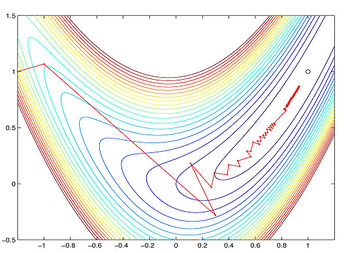
\includegraphics[width=5cm]{steepestDescent.jpg}
\end{center}

Iterate:
$$ \bfW_{k+1} = \bfW_k + \alpha \bfD, \quad \bfD =  -\grad E(\bfW_k). $$
Guaranteed to be a descent direction but need to make sure that
$$ E(\bfW_k + \alpha \bfD) < E(\bfW_k)  $$

\end{frame}

\begin{frame}
	\frametitle{Line Search Problem}
	\begin{center}
		\iwidth=40mm
		\iheight=30mm
		\begin{tabular}{cc}
			objective function
			&
			linesearch
			\\
			\scriptsize
			% This file was created by matlab2tikz.
% Minimal pgfplots version: 1.3
%
%The latest updates can be retrieved from
%  http://www.mathworks.com/matlabcentral/fileexchange/22022-matlab2tikz
%where you can also make suggestions and rate matlab2tikz.
%
\definecolor{mycolor1}{rgb}{0.00000,0.44700,0.74100}%
%

\begin{tikzpicture}

\begin{axis}[%
width=0.95092\iwidth,
height=\iheight,
at={(0\iwidth,0\iheight)},
scale only axis,
xmin=-1.5,
xmax=0.7,
ymin=-0.5,
ymax=0.5
]
\addplot[thick,contour prepared, contour prepared format=matlab, contour/labels=false,contour/draw color=black] table[row sep=crcr] {%
%
3.14929162120792	55\\
-0.206751084567955	-0.282608695652174\\
-0.256521739130435	-0.292968472312811\\
-0.352173913043478	-0.308800013833108\\
-0.447826086956522	-0.320023209776311\\
-0.543478260869565	-0.324868894870518\\
-0.639130434782609	-0.321114854585791\\
-0.734782608695652	-0.30598227359899\\
-0.810903690966283	-0.282608695652174\\
-0.830434782608696	-0.274633856633618\\
-0.889832393627909	-0.239130434782609\\
-0.926086956521739	-0.209639669767419\\
-0.939307382257738	-0.195652173913043\\
-0.970028854366405	-0.152173913043478\\
-0.991484708888687	-0.108695652173913\\
-1.00509639940392	-0.0652173913043478\\
-1.01170596423814	-0.0217391304347826\\
-1.01170596423814	0.0217391304347826\\
-1.00509639940392	0.0652173913043478\\
-0.991484708888687	0.108695652173913\\
-0.970028854366405	0.152173913043478\\
-0.939307382257738	0.195652173913043\\
-0.926086956521739	0.209639669767419\\
-0.889832393627909	0.239130434782609\\
-0.830434782608696	0.274633856633618\\
-0.810903690966283	0.282608695652174\\
-0.734782608695652	0.30598227359899\\
-0.639130434782609	0.321114854585791\\
-0.543478260869565	0.324868894870518\\
-0.447826086956522	0.320023209776311\\
-0.352173913043478	0.308800013833108\\
-0.256521739130435	0.292968472312811\\
-0.206751084567955	0.282608695652174\\
-0.160869565217391	0.272120335964711\\
-0.0652173913043479	0.246568933605764\\
-0.0407026156180396	0.239130434782609\\
0.0304347826086957	0.214870196619902\\
0.0817251657801165	0.195652173913043\\
0.126086956521739	0.176293105448535\\
0.176100681912772	0.152173913043478\\
0.221739130434783	0.12497807564539\\
0.246274477281357	0.108695652173913\\
0.292540981282389	0.0652173913043478\\
0.317141843086876	0.0217391304347826\\
0.317141843086876	-0.0217391304347826\\
0.292540981282389	-0.0652173913043478\\
0.246274477281358	-0.108695652173913\\
0.221739130434783	-0.12497807564539\\
0.176100681912772	-0.152173913043478\\
0.126086956521739	-0.176293105448535\\
0.0817251657801165	-0.195652173913043\\
0.0304347826086957	-0.214870196619902\\
-0.0407026156180398	-0.239130434782609\\
-0.0652173913043479	-0.246568933605764\\
-0.160869565217391	-0.272120335964711\\
-0.206751084567955	-0.282608695652174\\
3.73656931272967	83\\
-0.591170005980036	-0.456521739130435\\
-0.639130434782609	-0.460437052543239\\
-0.734782608695652	-0.462831462246709\\
-0.830434782608696	-0.458434588322427\\
-0.845299612486148	-0.456521739130435\\
-0.926086956521739	-0.443250631383436\\
-1.02173913043478	-0.414245783621238\\
-1.02445950378373	-0.41304347826087\\
-1.10228396758746	-0.369565217391304\\
-1.11739130434783	-0.358668303317297\\
-1.15258920869489	-0.326086956521739\\
-1.18936472851789	-0.282608695652174\\
-1.21304347826087	-0.246632183822474\\
-1.21716466023266	-0.239130434782609\\
-1.2360538856294	-0.195652173913043\\
-1.25032501848124	-0.152173913043478\\
-1.26057000658293	-0.108695652173913\\
-1.26719222171635	-0.0652173913043478\\
-1.27044298128662	-0.0217391304347826\\
-1.27044298128662	0.0217391304347826\\
-1.26719222171635	0.0652173913043478\\
-1.26057000658293	0.108695652173913\\
-1.25032501848124	0.152173913043478\\
-1.2360538856294	0.195652173913043\\
-1.21716466023266	0.239130434782609\\
-1.21304347826087	0.246632183822474\\
-1.18936472851789	0.282608695652174\\
-1.15258920869489	0.326086956521739\\
-1.11739130434783	0.358668303317297\\
-1.10228396758746	0.369565217391304\\
-1.02445950378373	0.41304347826087\\
-1.02173913043478	0.414245783621238\\
-0.926086956521739	0.443250631383436\\
-0.845299612486148	0.456521739130435\\
-0.830434782608696	0.458434588322427\\
-0.734782608695652	0.462831462246709\\
-0.639130434782609	0.460437052543239\\
-0.591170005980036	0.456521739130435\\
-0.543478260869565	0.452416983356333\\
-0.447826086956522	0.439502264614247\\
-0.352173913043478	0.423589542980075\\
-0.298083160445373	0.41304347826087\\
-0.256521739130435	0.404449857272025\\
-0.160869565217391	0.38213182356229\\
-0.110946370573327	0.369565217391304\\
-0.0652173913043479	0.357259343137234\\
0.0304347826086957	0.329974315084581\\
0.0431172908854798	0.326086956521739\\
0.126086956521739	0.298594912903262\\
0.172574819362186	0.282608695652174\\
0.221739130434783	0.264041392481254\\
0.284838937701467	0.239130434782609\\
0.317391304347826	0.22468652830333\\
0.379430049960013	0.195652173913043\\
0.41304347826087	0.17733052305253\\
0.456341054806181	0.152173913043478\\
0.508695652173913	0.114586593210819\\
0.516301394171093	0.108695652173913\\
0.554994098084705	0.0652173913043478\\
0.575356421826027	0.0217391304347826\\
0.575356421826027	-0.0217391304347826\\
0.554994098084705	-0.0652173913043478\\
0.516301394171093	-0.108695652173913\\
0.508695652173913	-0.114586593210819\\
0.456341054806181	-0.152173913043478\\
0.41304347826087	-0.17733052305253\\
0.379430049960013	-0.195652173913043\\
0.317391304347826	-0.224686528303329\\
0.284838937701467	-0.239130434782609\\
0.221739130434783	-0.264041392481254\\
0.172574819362186	-0.282608695652174\\
0.126086956521739	-0.298594912903262\\
0.0431172908854798	-0.326086956521739\\
0.0304347826086957	-0.329974315084581\\
-0.0652173913043479	-0.357259343137234\\
-0.110946370573327	-0.369565217391304\\
-0.160869565217391	-0.38213182356229\\
-0.256521739130435	-0.404449857272025\\
-0.298083160445374	-0.41304347826087\\
-0.352173913043478	-0.423589542980075\\
-0.447826086956522	-0.439502264614247\\
-0.543478260869565	-0.452416983356333\\
-0.591170005980036	-0.456521739130435\\
4.32384700425143	28\\
-1.22041279590659	-0.5\\
-1.28555999053104	-0.456521739130435\\
-1.30869565217391	-0.436949590946923\\
-1.33136607468592	-0.41304347826087\\
-1.36480702587585	-0.369565217391304\\
-1.39156601988892	-0.326086956521739\\
-1.40434782608696	-0.300357495765692\\
-1.41188848895528	-0.282608695652174\\
-1.42684599685359	-0.239130434782609\\
-1.43862956867932	-0.195652173913043\\
-1.44763786238666	-0.152173913043478\\
-1.4541616754961	-0.108695652173913\\
-1.45840417367997	-0.0652173913043478\\
-1.46049416948081	-0.0217391304347826\\
-1.46049416948081	0.0217391304347826\\
-1.45840417367997	0.0652173913043478\\
-1.4541616754961	0.108695652173913\\
-1.44763786238666	0.152173913043478\\
-1.43862956867932	0.195652173913043\\
-1.42684599685359	0.239130434782609\\
-1.41188848895528	0.282608695652174\\
-1.40434782608696	0.300357495765692\\
-1.39156601988892	0.326086956521739\\
-1.36480702587585	0.369565217391304\\
-1.33136607468592	0.41304347826087\\
-1.30869565217391	0.436949590946923\\
-1.28555999053104	0.456521739130435\\
-1.22041279590659	0.5\\
4.32384700425143	20\\
0.7	-0.116622219564237\\
0.653707982548674	-0.152173913043478\\
0.604347826086957	-0.182852313024265\\
0.582639903735045	-0.195652173913043\\
0.508695652173913	-0.23308811710231\\
0.496258375211213	-0.239130434782609\\
0.41304347826087	-0.275100367146866\\
0.395118957953456	-0.282608695652174\\
0.317391304347826	-0.312255544567221\\
0.280275828677267	-0.326086956521739\\
0.221739130434783	-0.346266041552522\\
0.153017252250318	-0.369565217391304\\
0.126086956521739	-0.378105678746463\\
0.0304347826086957	-0.40759564334024\\
0.0118999199515808	-0.41304347826087\\
-0.0652173913043479	-0.434416604435657\\
-0.146182314150482	-0.456521739130435\\
-0.160869565217391	-0.460325175408723\\
-0.256521739130435	-0.483245888107475\\
-0.32938645711486	-0.5\\
4.32384700425143	20\\
-0.32938645711486	0.5\\
-0.256521739130435	0.483245888107475\\
-0.160869565217391	0.460325175408723\\
-0.146182314150482	0.456521739130435\\
-0.0652173913043479	0.434416604435657\\
0.0118999199515812	0.41304347826087\\
0.0304347826086957	0.40759564334024\\
0.126086956521739	0.378105678746463\\
0.153017252250318	0.369565217391304\\
0.221739130434783	0.346266041552522\\
0.280275828677267	0.326086956521739\\
0.317391304347826	0.312255544567221\\
0.395118957953456	0.282608695652174\\
0.41304347826087	0.275100367146866\\
0.496258375211213	0.239130434782609\\
0.508695652173913	0.23308811710231\\
0.582639903735045	0.195652173913043\\
0.604347826086957	0.182852313024265\\
0.653707982548674	0.152173913043478\\
0.7	0.116622219564237\\
4.91112469577318	2\\
-1.46726630501234	-0.5\\
-1.5	-0.460858568944326\\
4.91112469577318	16\\
0.7	-0.218075100682267\\
0.659079762892463	-0.239130434782609\\
0.604347826086957	-0.264187205822476\\
0.563137036683871	-0.282608695652174\\
0.508695652173913	-0.304767699714434\\
0.455508468937322	-0.326086956521739\\
0.41304347826087	-0.341832507610435\\
0.337624562697656	-0.369565217391304\\
0.317391304347826	-0.376524628963239\\
0.221739130434783	-0.408962941233904\\
0.209361374264266	-0.41304347826087\\
0.126086956521739	-0.438929696483417\\
0.0693581468831773	-0.456521739130435\\
0.0304347826086957	-0.467970601529935\\
-0.0652173913043479	-0.495732852522326\\
-0.0806332257682523	-0.5\\
4.91112469577318	2\\
-1.5	0.460858568944326\\
-1.46726630501234	0.5\\
4.91112469577318	16\\
-0.0806332257682523	0.5\\
-0.0652173913043479	0.495732852522326\\
0.0304347826086957	0.467970601529935\\
0.0693581468831773	0.456521739130435\\
0.126086956521739	0.438929696483417\\
0.209361374264266	0.41304347826087\\
0.221739130434783	0.408962941233904\\
0.317391304347826	0.376524628963239\\
0.337624562697656	0.369565217391304\\
0.41304347826087	0.341832507610435\\
0.455508468937322	0.326086956521739\\
0.508695652173913	0.304767699714434\\
0.563137036683871	0.282608695652174\\
0.604347826086957	0.264187205822476\\
0.659079762892463	0.239130434782609\\
0.7	0.218075100682268\\
5.49840238729494	12\\
0.7	-0.283895926097209\\
0.604347826086957	-0.32387289166708\\
0.598965518855474	-0.326086956521739\\
0.508695652173913	-0.360436930863112\\
0.484574138075716	-0.369565217391304\\
0.41304347826087	-0.394885677937617\\
0.361757023015477	-0.41304347826087\\
0.317391304347826	-0.427854658852314\\
0.231920943058537	-0.456521739130435\\
0.221739130434783	-0.459760899049106\\
0.126086956521739	-0.489477964908959\\
0.0920097940282215	-0.5\\
5.49840238729494	12\\
0.0920097940282215	0.5\\
0.126086956521739	0.489477964908959\\
0.221739130434783	0.459760899049106\\
0.231920943058537	0.456521739130435\\
0.317391304347826	0.427854658852314\\
0.361757023015477	0.41304347826087\\
0.41304347826087	0.394885677937617\\
0.484574138075716	0.369565217391304\\
0.508695652173913	0.360436930863112\\
0.598965518855474	0.326086956521739\\
0.604347826086957	0.32387289166708\\
0.7	0.283895926097209\\
6.08568007881669	9\\
0.7	-0.333789281057698\\
0.609332765061261	-0.369565217391304\\
0.604347826086957	-0.371405121352418\\
0.508695652173913	-0.406240483549502\\
0.489962569982966	-0.41304347826087\\
0.41304347826087	-0.439382924831634\\
0.363344635574781	-0.456521739130435\\
0.317391304347826	-0.471552842573921\\
0.231337890620984	-0.5\\
6.08568007881669	9\\
0.231337890620984	0.5\\
0.317391304347826	0.471552842573921\\
0.363344635574781	0.456521739130435\\
0.41304347826087	0.439382924831634\\
0.489962569982966	0.41304347826087\\
0.508695652173913	0.406240483549502\\
0.604347826086957	0.371405121352418\\
0.609332765061261	0.369565217391304\\
0.7	0.333789281057698\\
6.67295777033845	7\\
0.7	-0.375851223701105\\
0.604347826086957	-0.411786696643559\\
0.600957310296833	-0.41304347826087\\
0.508695652173913	-0.445291041817953\\
0.476849761544354	-0.456521739130435\\
0.41304347826087	-0.477864772204736\\
0.347694036846476	-0.5\\
6.67295777033845	7\\
0.347694036846476	0.5\\
0.41304347826087	0.477864772204736\\
0.476849761544354	0.456521739130435\\
0.508695652173913	0.445291041817953\\
0.600957310296833	0.41304347826087\\
0.604347826086957	0.411786696643559\\
0.7	0.375851223701105\\
7.2602354618602	6\\
0.7	-0.412549194057046\\
0.698688510239842	-0.41304347826087\\
0.604347826086957	-0.446570305181768\\
0.576635910045962	-0.456521739130435\\
0.508695652173913	-0.479662928042734\\
0.449824088571756	-0.5\\
7.2602354618602	6\\
0.449824088571756	0.5\\
0.508695652173913	0.479662928042734\\
0.576635910045962	0.456521739130435\\
0.604347826086957	0.446570305181768\\
0.698688510239842	0.41304347826087\\
0.7	0.412549194057046\\
7.84751315338196	4\\
0.7	-0.444067149072774\\
0.665824109097759	-0.456521739130435\\
0.604347826086957	-0.477771622974777\\
0.541019830544344	-0.5\\
7.84751315338196	4\\
0.541019830544344	0.5\\
0.604347826086957	0.477771622974777\\
0.665824109097759	0.456521739130435\\
0.7	0.444067149072774\\
8.43479084490372	2\\
0.7	-0.472893053857135\\
0.623769614299825	-0.5\\
8.43479084490372	2\\
0.623769614299825	0.5\\
0.7	0.472893053857135\\
};
\addplot [very thick,color=black,only marks,mark=o,mark options={solid},forget plot]
  table[row sep=crcr]{%
-0.34657	0\\
};
\addplot [very thick,color=blue,only marks,mark=o,mark options={solid},forget plot]
  table[row sep=crcr]{%
0.5	0.4\\
};
\addplot [very thick,color=red,solid,forget plot]
  table[row sep=crcr]{%
0.5	0.4\\
0.195732495379911	-0.447007252408304\\
};
\addplot [very thick,color=red,only marks,mark=square,mark options={solid},forget plot]
  table[row sep=crcr]{%
0.344823572643755	-0.0319736987282349\\
};
\addplot [very thick,color=blue,only marks,mark=square,mark options={solid},forget plot]
  table[row sep=crcr]{%
0.195732495379911	-0.447007252408304\\
};
\end{axis}
\end{tikzpicture}%
			&
			\scriptsize
			% This file was created by matlab2tikz.
% Minimal pgfplots version: 1.3
%
%The latest updates can be retrieved from
%  http://www.mathworks.com/matlabcentral/fileexchange/22022-matlab2tikz
%where you can also make suggestions and rate matlab2tikz.
%
\definecolor{mycolor1}{rgb}{0.00000,0.44700,0.74100}%
%

\begin{tikzpicture}

\begin{axis}[%
width=0.95092\iwidth,
height=\iheight,
at={(0\iwidth,0\iheight)},
scale only axis,
xmin=0,
xmax=0.9,
ymin=3,
ymax=6
]
\addplot [very thick,color=red,solid,forget plot]
  table[row sep=crcr]{%
0	5.95117302460636\\
0.009	5.82406697744345\\
0.018	5.70109351561337\\
0.027	5.58214851987066\\
0.036	5.46713105569809\\
0.045	5.35594328993058\\
0.054	5.24849040985294\\
0.063	5.14468054470484\\
0.072	5.04442468952876\\
0.081	4.94763663129835\\
0.09	4.85423287726639\\
0.099	4.7641325854736\\
0.108	4.67725749736093\\
0.117	4.59353187242994\\
0.126	4.51288242489724\\
0.135	4.43523826229085\\
0.144	4.36053082593768\\
0.153	4.28869383329279\\
0.162	4.21966322206288\\
0.171	4.15337709607743\\
0.18	4.08977567286272\\
0.189	4.02880123287509\\
0.198	3.97039807035105\\
0.207	3.91451244573345\\
0.216	3.86109253963376\\
0.225	3.81008840829202\\
0.234	3.76145194049718\\
0.243	3.71513681593147\\
0.252	3.67109846490388\\
0.261	3.62929402943869\\
0.27	3.58968232568616\\
0.279	3.55222380762352\\
0.288	3.51688053201539\\
0.297	3.48361612460373\\
0.306	3.45239574749845\\
0.315	3.42318606774071\\
0.324	3.39595522701175\\
0.333	3.37067281246125\\
0.342	3.34730982862973\\
0.351	3.32583867044071\\
0.36	3.30623309723883\\
0.369	3.28846820785128\\
0.378	3.27252041665041\\
0.387	3.25836743059624\\
0.396	3.24598822723843\\
0.405	3.23536303365787\\
0.414	3.22647330632888\\
0.423	3.21930171188363\\
0.432	3.21383210876102\\
0.441	3.21004952972323\\
0.45	3.2079401652233\\
0.459	3.20749134760827\\
0.468	3.20869153614261\\
0.477	3.21153030283758\\
0.486	3.21599831907255\\
0.495	3.22208734299511\\
0.504	3.229790207687\\
0.513	3.23910081008408\\
0.522	3.25001410063839\\
0.531	3.26252607371138\\
0.54	3.27663375868784\\
0.549	3.29233521180041\\
0.558	3.3096295086552\\
0.567	3.32851673744959\\
0.576	3.34899799287357\\
0.585	3.37107537068677\\
0.594	3.39475196296355\\
0.603	3.42003185399901\\
0.612	3.44692011686944\\
0.621	3.47542281064108\\
0.63	3.50554697822124\\
0.639	3.53730064484687\\
0.648	3.57069281720544\\
0.657	3.60573348318397\\
0.666	3.64243361224205\\
0.675	3.68080515640548\\
0.684	3.72086105187721\\
0.693	3.76261522126308\\
0.702	3.80608257640977\\
0.711	3.8512790218533\\
0.72	3.89822145887643\\
0.729	3.94692779017381\\
0.738	3.99741692512432\\
0.747	4.04970878567002\\
0.756	4.10382431280202\\
0.765	4.15978547365344\\
0.774	4.21761526920056\\
0.783	4.27733774257306\\
0.792	4.33897798797521\\
0.801	4.40256216021969\\
0.81	4.46811748487666\\
0.819	4.53567226904052\\
0.828	4.60525591271763\\
0.837	4.67689892083836\\
0.846	4.75063291589732\\
0.855	4.826490651226\\
0.864	4.90450602490236\\
0.873	4.98471409430244\\
0.882	5.06715109129913\\
0.891	5.15185443811404\\
0.9	5.23886276382841\\
};
\addplot [very thick, color=blue,only marks,mark=o,mark options={solid},forget plot]
  table[row sep=crcr]{%
0	5.95117302460636\\
};
\addplot [very thick, color=red,only marks,mark=square,mark options={solid},forget plot]
  table[row sep=crcr]{%
0.459	3.20749134760827\\
};
\addplot [very thick, color=blue,only marks,mark=square,mark options={solid},forget plot]
  table[row sep=crcr]{%
0.9	5.23886276382841\\
};
\end{axis}
\end{tikzpicture}%
		\end{tabular}
	\end{center}
	Let $E$ be the cross entropy, $\bfW_k$ the current weights, and $\bfD$ the search direction.  The line search problem is:
	\begin{equation*}
		\min_{\alpha > 0} \phi(\alpha) \quad \text{ where } \quad \phi(\alpha) = E(\bfW_k + \alpha \bfD).
	\end{equation*}
\end{frame}


\begin{frame}\frametitle{Armijo Line Search}

A method for inexact line search


\begin{itemize}
\item Start with $\alpha = \alpha_0$
\item Test $ E(\bfW + \alpha \bfD) {<} E(\bfW)$
\item If fail $\alpha \leftarrow \hf \alpha$
\end{itemize}

\bigskip
\pause

A few (small) but helpful tricks
\begin{itemize}
\item Choose your $\alpha_0$ based on the problem
\item If line search is needed ($\alpha\not=\alpha_0$) at iteration $k$ set $\alpha_0 = \alpha_k$ in next iteration.
\item If no line search is needed ($\alpha =\alpha_0$) at iteration $k$ set $\alpha_0 = \gamma\alpha_k$, $\gamma>1$ in next iteration.
\end{itemize}


\end{frame}


\begin{frame}[fragile]\frametitle{Coding: Steepest Descent }

Write a code for steepest descent with Armijo linesearch.

\begin{verbatim}
function W = steepestDescent(E,W,param)
% Inputs:
%     E  - function that provides value and gradient
%     W  - starting guess
%  param - struct with parameters

alpha     = param.maxStep; % max step size
maxIter   = param.maxIter; % max number of iterations

for i=1:maxIter

% Your code here
end
\end{verbatim}

\end{frame}



\begin{frame}[allowframebreaks]
	\frametitle{References}
\bibliographystyle{abbrv}
 % \bibliographystyle{plainnat}
\bibliography{NumDNN}

\end{frame}

\end{document}













